\documentclass{article}
\usepackage{graphicx} % Required for inserting images

\title{Ultrahangos mérés}
\author{Kern Luca, Csongor Vincze}
\date{2026 Február 25}

\begin{document}

\maketitle

\section{1. Feladat Ismerkedés az oszcilloszkóp és a függvénygenerátor használatával.}

Beállítottuk a 4 V amplitúdójú, 1 V eltolású 115 Hz-es szinuszjelet. Csatlakoztattuk a jelet az oszcilloszkóphoz is. Beállítottuk a triggert, és stabilizáltuk, ízlésesen a képernyő közepér hoztuk a jelet.
Végül közelítőleg lemértük a jel amplitúdóját és frekvenciáját.

\begin{table}[h!]
    \centering
    \begin{tabular}{|l|c|c|}
        \hline
        Paraméter & Beállított érték & kurzorral mért érték & funkcióval mért érték \\ \hline
        Amplitúdó 4,0 ?? & 4,0 & 4,0 \\ \hline
        Frekvencia 115,0 & 116,3 & 114,9 \\ \hline
    \end{tabular}
    \caption{A beállított és a mért amplitúdó és frekvencia értékek.}
    \label{tab:amplitudo_frekvencia}
\end{table}

A különbség az RMS és a csúcstól csúcsig mért értékek között a fő különbség, hogy a csúcstól csúcsig mért érték az amplitúdó kétszerese, míg az effektív érték a jel négyzetének a kiátlagolásának a gyöke.

Megváltoztattuk a csatolási módot DC-ről AC-re, így kiküszöböltük a konstans tagú feszültség miatti eltolást.
Ha a csatolást "Ground"-ra állítottuk a következő történt:

Végül a kurzor egyenesek segítségével is megmértük az amplitúdó és frekvencia értékeit a jelnek.


\begin{figure}[htp]
    \centering
    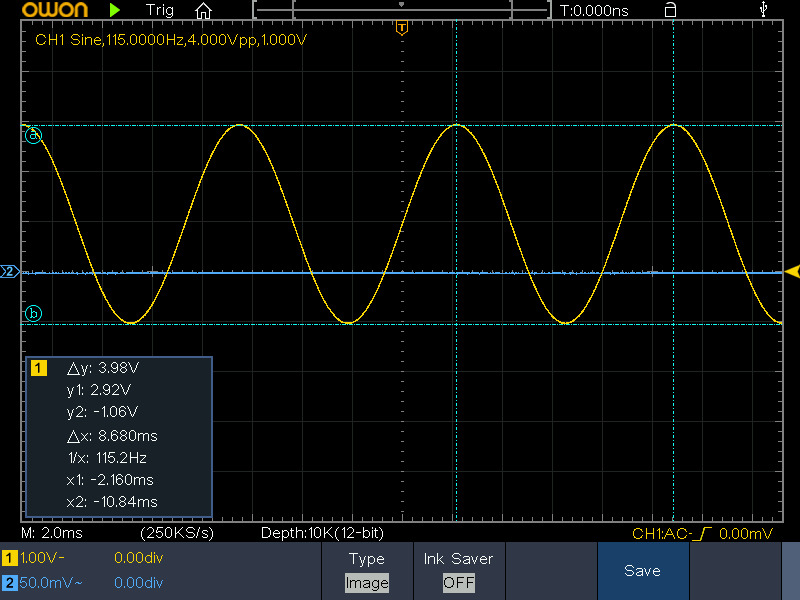
\includegraphics[width=4cm]{1.42.jpg}
    \caption{Az oszcilloszkóp különböző funkcióinak kipróbálása}
    \label{probalkozas}
\end{figure}

\section{Ultrahangos adó-vevő páros átviteli karakterisztikája
a frekvencia függvényében}

Lehelyeztük a két adó-vevőt körülbelül 10 cm távolságra, és kissé elforgattuk őket, hogy ne zavarjanak be a visszaverődő hullámok. Ezután beállítottuk az 6 V-os eltolásmentes színuszjelet. Csatlakoztattuk az koax kábelt a jelgenerátorhoz, aztán egy koaxkábeles elosztóval bekötöttük a jelet az oszcilloszkópba és az adóba is. Az oszcilloszkóp másik bemenetéhez pedig csatlakoztattuk a vevőt. Ezután beállítottuk a triggert.

\begin{table}[h!]
    \centering
    \begin{tabular}{|c|c|}
        \hline
        Frekvencia [kHz] & Amplitúdó [mV] \\ \hline
        1 & 0 \\ \hline 
        5 & 0\\ \hline
        10 & 0\\ \hline 
        15 & 0\\ \hline
        20 & 0\\ \hline
        25 & 0\\ \hline
        30 & 0\\ \hline
        35 & 3 \\ \hline
        40 & 183\\ \hline
        45 & 15\\ \hline
        50 & 12\\ \hline
        51,9 & 19\\ \hline
        55 & 2\\ \hline
        60 & 1\\ \hline
        65 & 2\\ \hline
        70 & 1\\ \hline
        75 & 1\\ \hline
        80 & 1\\ \hline
        85 & 1\\ \hline
        90 & 1\\ \hline
        95 & 2\\ \hline
        93,5 & 2\\ \hline
        100 & 1\\ \hline
    \end{tabular}
    \caption{Az adó-vevő páros átviteli karakterisztikájának mérési adatai.}
    \label{tab:atviteli_karakterisztika}
\end{table}


\begin{enumerate}
    \item A legalacsonyabb frekvenciájú jel, amit ezzel a beállítással mérni lehet: 
    \item A frekvencia, amitől kezdve hallani kezdjük a jelet: 5kHz
    \item A legmagasabb frekvencia, amit még hallunk: 17,4kHz
    \item A rezonanciafrekvenciák: 40,27 kHz (itt 179,1 mV ampilitúdót mértünk), 51,9 kHz (itt 19 mV  volt), 93,5 kHz (itt 2,6 mV volt a mért adat)
    \item A rezonanciafrekvencia, amely a legnagyobb csúcsot adja: 40,27 kHz, itt a csúcs 179,1 mV volt
\end{enumerate}


\begin{table}[h!]
    \centering
    \begin{tabular}{|c|c|}
        \hline
        Frekvencia [kHz] & Amplitúdó [mV] \\ \hline
        38,0 & 32,8 \\ \hline
        39,0 & 70,2 \\ \hline
        39,2 & 82,1 \\ \hline
        39,4 & 99,0 \\ \hline
        39,6 & 121,3 \\ \hline
        39,8 & 148,4 \\ \hline
        40,0 & 160,2 \\ \hline
        40,2 & 176,6 \\ \hline
        40,23 & 173,3 \\ \hline
        40,25 & 178,8 \\ \hline
        40,26 & 178,3 \\ \hline
        40,27 & 179,1 \\ \hline
        40,28 & 178,6 \\ \hline
        40,29 & 179,0 \\ \hline
        40,3 & 176,6 \\ \hline
        40,4 & 174,4 \\ \hline
        40,5 & 16,3 \\ \hline
        41,0 & 152,4 \\ \hline
    \end{tabular}
    \caption{Rezonanciafrekvencia körüli adatpontok.}
    \label{rezonancia freki}
\end{table}


A rezonanciafrekvencia értéke:


\begin{table}[h!]
    \centering
    \begin{tabular}{|c|c|}
        \hline
        Frekvencia [kHz] & Amplitúdó [V] \\ \hline
         &  \\ \hline
         &  \\ \hline
         &  \\ \hline
         &  \\ \hline
         &  \\ \hline

         &  \\ \hline
         &  \\ \hline
         &  \\ \hline
         &  \\ \hline
         &  \\ \hline
    \end{tabular}
    \caption{Csúcstól csúcsig amplitúdó értékek}
    \label{Vpp}
\end{table}


\section{Hangsebesség meghatározása az átvitt jel fázisának mérésével}


\begin{table}[h!]
    \centering
    \begin{tabular}{|c|c|c|}
        \hline
        Távolság [mm] & Idő & Sebesség \\ \hline
        0 & & \\ \hline
        2 & & \\ \hline
        4 & & \\ \hline
        6 & & \\ \hline
        8 & & \\ \hline
        10 & & \\ \hline
        12 & & \\ \hline
        14 & & \\ \hline
        16 & & \\ \hline
        18 & & \\ \hline
        20 & & \\ \hline
        22 & & \\ \hline
        24 & & \\ \hline
    \end{tabular}
    \caption{A hangsebesség mérése a távolság függvényében.}
    \label{tab:hangsebesseg_meres}
\end{table}

A hullámhossz:

\begin{figure}[htp]
    \centering
    % \includegraphics[width=4cm]{your_image_here.png}
    \caption{Az oszcilloszkóp különböző funkcióinak kipróbálása}
    \label{hangsebesség_grafikon}
\end{figure}


\section{Állóhullám mintázat}



\begin{table}[h!]
    \centering
    \begin{tabular}{|c|c|c|}
        \hline
        Távolság [mm] & Amplitúdó \\ \hline
        0 &  \\ \hline
        2 &  \\ \hline
        4 &  \\ \hline
        6 &  \\ \hline
        8 &  \\ \hline
        10 &  \\ \hline
        12 &  \\ \hline
        14 &  \\ \hline
        16 &  \\ \hline
        18 &  \\ \hline
        20 &  \\ \hline
        22 &  \\ \hline
        24 &  \\ \hline
    \end{tabular}
    \caption{állóhullám amplitúdófüggese a távoldágtól}
    \label{állóhullám}
\end{table}


Utolagosan ujramerve a rezonanciafrekvencia 40,81kHznek adódott, 0,01kHzes mozgatással határoztam meg.





\end{document}